% !TEX root = thesis.tex

\chapter{Hotels-50K}
\label{ch:4}

% hotels-50K


The Hotels-50K dataset is a carefully curated subset of the data collected both using teh TraffickCam application and publicly available data. The Hotels-50K dataset includes over 1 million images from 50,000 hotels around the world, and is designed to support efforts by the broader computer vision community to address the challenging hotel recognition task.

In our presentation of the Hotels-50K dataset, we first propose and formulate the problem of hotel instance recognition.  Second, we curate and share a data set and evaluation protocol for this problem at a scale that is relevant to international efforts to address trafficking.  Third, we describe and test algorithms that include the data augmentation steps necessary to attack this problem as a reasonable baseline for comparisons.

\begin{figure}
    \centering
    \includegraphics[height=1.8in]{figures/example_images/queries/1.png}
    \includegraphics[height=1.8in]{figures/example_images/queries/2.png}
    \includegraphics[height=1.8in]{figures/example_images/queries/3.png}
    \caption{Example images from hotel rooms used in human trafficking investigations with the region containing the victim masked off.}
    \label{fig:queries}
\end{figure}

\section{Related Work}
Hotels-50k is a large-scale dataset designed to support research in hotel recognition
for images with the long term goal of supporting robust applications to aid in criminal
investigations. In this section, we review related efforts towards (1) AI to combat human trafficking, (2) targeted large-scale image datasets, and (3) scene and place recognition.

\paragraph{AI to Combat Human Trafficking.} The Hotels-50K dataset and the problem of automatically recognizing hotel rooms fits within a larger set of efforts to apply machine learning, computer vision, and natural language processing to the domain of addressing human trafficking.  These efforts largely focused on indexing online escort advertisements, based on locations and phone numbers in the advertisement text or imprinted on advertising images~\cite{alvari2017semi,dubrawski2015leveraging,kejriwal2017investigative,szekely2015building}.  Additionally, there are larger-scale projects, such as Thorn\footnote{\url{https://www.wearethorn.org/}} that implement approaches including facial identification for identifying victims of child sex trafficking and sexual abuse.


\paragraph{Targeted Large-Scale Image Datasets} The computer vision community has a long tradition of developing datasets to support and challenge the research community. Some of most well-known datasets include ImageNet~\cite{deng2009imagenet}, Places~\cite{zhou2017places}, and CIFAR-100~\cite{krizhevsky2009learning}.
These benchmarks drive competitions for comparing classification and retrieval methods, but because they tend to focus on general (unrelated) categories of images there have been additional efforts towards curating domain-specific datasets, including datasets of classes of cars~\cite{CAR196} and birds~\cite{wah2011caltech}.  Most closely related to Hotels-50K are datasets that directly address investigative use-cases, including a database of tattoos~\cite{ngan2015tattoo}, and a dataset of advertisements labelled by whether they include a victim of trafficking~\cite{tong2017combating}. 

%moved this figure far forward to fix problems later.
\begin{figure}
    \centering
    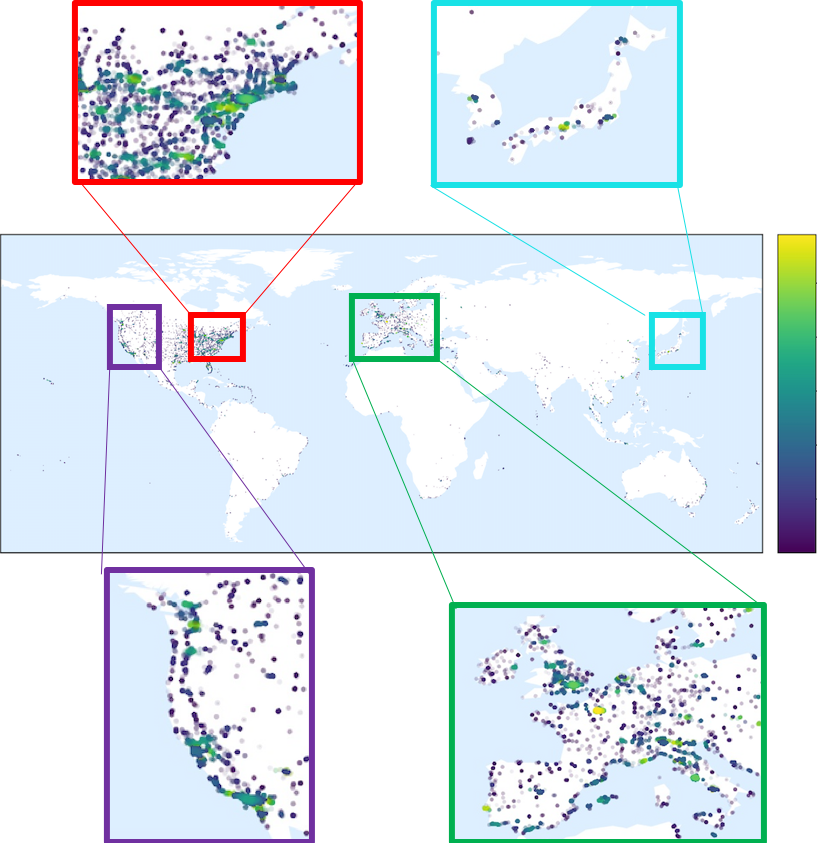
\includegraphics[width=.95\columnwidth]{figures/geographic_hist/geographic_density2.png}
    \caption{Geographic distribution of the Hotels-50K dataset, with a dot at every hotel location, color coded (from blue to yellow) by the local density of hotels. Images are most abundant in the United States, Western Europe and along popular coastlines. }
    \label{fig:geographicDensity}
\end{figure}

\paragraph{Scene and Place Recognition}
Recognizing the scene from which an image was captured has been a problem of great interest in the computer vision community. Most work in this area focuses on the problem of identifying the scene category (e.g., park, beach, parking lot) rather than particular locations, but recently there has been increased interest in estimating the precise geographic location of an image.

This place recognition problem can also be formulated as an image retrieval task where geotagged images serve as a database, and a query image's location is inferred by finding visually similar images in the dataset~\cite{baatz2012large,chen2011city,crandall2009mapping,hays2008im2gps,jacobs07geolocate,schindler2007city,torii2013visual,zamir2010accurate,googleLandmarks}. Increasingly, methods train deep neural networks to produce similar features for images from nearby locations~\cite{zhou2014recognizing,netvlad,visualPlaceRecognition,vo2017revisit,zhai2018geotemporal}.  

\newcommand{\exampleImWidth}{1in}
\newcommand{\exampleImHeight}{.65in}
\begin{figure*}
    \begin{tabular}{ccc|ccc}

        \multicolumn{3}{c|}{(a) Travel Websites} & \multicolumn{3}{c}{(b) TraffickCam} \\

        \raisebox{-.5\height}{\includegraphics[width=\exampleImWidth]{figures/example_images/expedia/6/1.jpg}}
        &
        \raisebox{-.5\height}{\includegraphics[width=\exampleImWidth]{figures/example_images/expedia/6/2.jpg}}
        &
        \raisebox{-.5\height}{\includegraphics[width=\exampleImWidth]{figures/example_images/expedia/6/3.jpg}}
        &
        \raisebox{-.5\height}{\includegraphics[width=\exampleImWidth]{figures/example_images/tcam/6/2.jpg}}
        & 
        \raisebox{-.5\height}{\includegraphics[width=.6in]{figures/example_images/tcam/6/1.jpg}}
        & 
        \raisebox{-.5\height}{\includegraphics[width=.6in]{figures/example_images/tcam/6/3.jpg}}
        
        \\
        \hline
        
        \raisebox{-.5\height}{\includegraphics[width=\exampleImWidth]{figures/example_images/expedia/10/1.jpg}}
        &
        \raisebox{-.5\height}{\includegraphics[width=\exampleImWidth]{figures/example_images/expedia/10/2.jpg}}
        &
        \raisebox{-.5\height}{\includegraphics[width=\exampleImWidth]{figures/example_images/expedia/10/3.jpg}}
        &
        \raisebox{-.5\height}{\includegraphics[width=\exampleImWidth]{figures/example_images/tcam/10/2.jpg}}
        & 
        \raisebox{-.5\height}{\includegraphics[width=.6in]{figures/example_images/tcam/10/1.jpg}}
        & 
        \raisebox{-.5\height}{\includegraphics[width=.6in]{figures/example_images/tcam/10/3.jpg}} 
        
        % \\
        % \hline

        % \raisebox{-.5\height}{\includegraphics[width=\exampleImWidth]{figures/example_images/expedia/1/1.png}}
        % & 
        % \raisebox{-.5\height}{\includegraphics[width=\exampleImWidth]{figures/example_images/expedia/1/3.png}}
        % & 
        % \raisebox{-.5\height}{\includegraphics[width=.65in]{figures/example_images/expedia/1/2.png}} 
        % &
        % \raisebox{-.5\height}{\includegraphics[width=\exampleImWidth]{figures/example_images/tcam/1/1.png}}
        % &
        % \raisebox{-.5\height}{\includegraphics[width=\exampleImWidth]{figures/example_images/tcam/1/2.png}}
        % &
        % \raisebox{-.5\height}{\includegraphics[width=.6in]{figures/example_images/tcam/1/3.png}} 
        
        \\
        \hline
        
        \raisebox{-.5\height}{\includegraphics[width=.96in]{figures/example_images/expedia/4/1.jpg}}
        &
        \raisebox{-.5\height}{\includegraphics[width=.95in]{figures/example_images/expedia/4/2.jpg}}
        &
        \raisebox{-.5\height}{\includegraphics[width=\exampleImWidth]{figures/example_images/expedia/4/3.jpg}}
        &
        \raisebox{-.5\height}{\includegraphics[width=\exampleImWidth]{figures/example_images/tcam/4/2.jpg}}
        &
        \raisebox{-.5\height}{\includegraphics[width=\exampleImWidth]{figures/example_images/tcam/4/3.jpg}}
        &
        \raisebox{-.5\height}{\includegraphics[width=.6in]{figures/example_images/tcam/4/1.jpg}}
        
        \\
        \hline

        \raisebox{-.5\height}{\includegraphics[width=\exampleImWidth]{figures/example_images/expedia/5/1.jpg}}
        &
        \raisebox{-.5\height}{\includegraphics[width=\exampleImWidth]{figures/example_images/expedia/5/2.jpg}}
        &
        \raisebox{-.5\height}{\includegraphics[width=\exampleImWidth]{figures/example_images/expedia/5/3.jpg}}
        & 
        \raisebox{-.5\height}{\includegraphics[width=\exampleImWidth]{figures/example_images/tcam/5/1.jpg}}
        &
        \raisebox{-.5\height}{\includegraphics[width=\exampleImWidth]{figures/example_images/tcam/5/2.jpg}}
        & 
        \raisebox{-.5\height}{\includegraphics[width=.6in]{figures/example_images/tcam/5/3.jpg}} 
        
        % \\
        % \hline

        % \raisebox{-.5\height}{\includegraphics[width=\exampleImWidth]{figures/example_images/expedia/7/1.jpg}}
        % &
        % \raisebox{-.5\height}{\includegraphics[width=\exampleImWidth]{figures/example_images/expedia/7/2.jpg}}
        % &
        % \raisebox{-.5\height}{\includegraphics[width=\exampleImWidth]{figures/example_images/expedia/7/3.jpg}}
        % &
        % \raisebox{-.5\height}{\includegraphics[width=\exampleImWidth]{figures/example_images/tcam/7/2.jpg}}
        % & 
        % \raisebox{-.5\height}{\includegraphics[width=\exampleImWidth]{figures/example_images/tcam/7/3.jpg}} 
        % & 
        % \raisebox{-.5\height}{\includegraphics[width=.6in]{figures/example_images/tcam/7/1.jpg}}
        
        % \\
        % \hline
        
        %  \raisebox{-.5\height}{\includegraphics[width=\exampleImWidth]{figures/example_images/expedia/2/1.jpg}} & 
        %  \raisebox{-.5\height}{\includegraphics[width=\exampleImWidth]{figures/example_images/expedia/2/2.jpg}}
        %  &
        %  \raisebox{-.5\height}{\includegraphics[width=\exampleImWidth]{figures/example_images/expedia/2/3.jpg}} &
        %  \raisebox{-.5\height}{\includegraphics[width=\exampleImWidth]{figures/example_images/tcam/2/1.jpg}}
        %  &
        %  \raisebox{-.5\height}{\includegraphics[width=\exampleImWidth]{figures/example_images/tcam/2/2.jpg}}
        %  &
        %  \raisebox{-.5\height}{\includegraphics[width=\exampleImWidth]{figures/example_images/tcam/2/3.jpg}}
         
        % \\
        % \hline

        % \raisebox{-.5\height}{\includegraphics[width=\exampleImWidth]{figures/example_images/expedia/3/1.jpg}}
        % &
        % \raisebox{-.5\height}{\includegraphics[width=\exampleImWidth]{figures/example_images/expedia/3/2.jpg}}
        % &
        % \raisebox{-.5\height}{\includegraphics[width=\exampleImWidth]{figures/example_images/expedia/3/3.jpg}}
        % &
        % \raisebox{-.5\height}{\includegraphics[width=\exampleImWidth]{figures/example_images/tcam/3/1.jpg}}
        % &
        % \raisebox{-.5\height}{\includegraphics[width=\exampleImWidth]{figures/example_images/tcam/3/2.jpg}}
        % &
        % \raisebox{-.5\height}{\includegraphics[width=\exampleImWidth]{figures/example_images/tcam/3/3.jpg}}
        
        % \\
        % \hline
        

        % \raisebox{-.5\height}{\includegraphics[width=\exampleImWidth]{figures/example_images/expedia/8/1.jpg}}
        % &
        % \raisebox{-.5\height}{\includegraphics[width=\exampleImWidth]{figures/example_images/expedia/8/2.jpg}}
        % &
        % \raisebox{-.5\height}{\includegraphics[width=\exampleImWidth]{figures/example_images/expedia/8/3.jpg}}
        % & 
        % \raisebox{-.5\height}{\includegraphics[width=\exampleImWidth]{figures/example_images/tcam/8/1.jpg}}
        % &
        % \raisebox{-.5\height}{\includegraphics[width=\exampleImWidth]{figures/example_images/tcam/8/2.jpg}}
        % & 
        % \raisebox{-.5\height}{\includegraphics[width=\exampleImWidth]{figures/example_images/tcam/8/3.jpg}} 
        
        % \\
        % \hline
        

        % \raisebox{-.5\height}{\includegraphics[width=\exampleImWidth]{figures/example_images/expedia/9/1.jpg}}
        % &
        % \raisebox{-.5\height}{\includegraphics[width=\exampleImWidth]{figures/example_images/expedia/9/2.jpg}}
        % &
        % \raisebox{-.5\height}{\includegraphics[width=\exampleImWidth]{figures/example_images/expedia/9/3.jpg}}
        % & 
        % \raisebox{-.5\height}{\includegraphics[width=\exampleImWidth]{figures/example_images/tcam/9/1.jpg}}
        % &
        % \raisebox{-.5\height}{\includegraphics[width=\exampleImWidth]{figures/example_images/tcam/9/2.jpg}}
        % & 
        % \raisebox{-.5\height}{\includegraphics[width=\exampleImWidth]{figures/example_images/tcam/9/3.jpg}} 
    \end{tabular}
    \caption[Image variability from different sources]{Comparing images across data sources shows clear differences in image quality and lighting.  Each row shows images from the same hotel, with examples from (a) travel websites and (b) the TraffickCam crowd-sourcing app.}
    \label{fig:domainImages}
\end{figure*}

Algorithms trying recognize a specific place can exploit the fact that the same objects or landmarks appear in the same geometric configuration from different viewpoints. These geometric and matching approaches do not apply to hotel recognition.
Within a hotel, the rooms may have some objects that are the same (e.g., every room has the same headboard), some objects that are different (e.g., different artwork on the walls), and those objects may be in different configurations from room to room (e.g., two beds vs. one or furniture on different walls).

\paragraph{Summary} Hotels-50K follows in the tradition of large-scale datasets widely used in the computer vision and machine learning communities. This dataset will support and complement the recent trend for using AI to combat criminal activity, specifically human trafficking. The problem of hotel recognition poses unique challenges and existing methods designed for recognizing outdoor scenes or landmarks are not well-suited to the problem of discriminating between similar-looking hotel rooms. 

\section{The Hotels-50K Dataset}

Hotels-50K consists of 1,027,871 images from 50,000 unique hotels around the world. 
Each of the images in the Hotels-50K dataset includes the following metadata: (1) hotel name, (2) geographic location, and (3) hotel chain, or \emph{Other} if the hotel property is not part of a major chain.

Figure~\ref{fig:geographicDensity} shows the geographic distribution of the images in our dataset. While the dataset consists of images from around the world, the images are more densely captured in the United States, Western Europe, and coastal regions.

\paragraph{Data Sources} The images in Hotels-50K come from two primary sources: (1) scraped from publicly available travel websites, such as Expedia and (2) captured by the crowdsourcing mobile application, TraffickCam, which allows travelers to submit photos of their hotel room. Figure~\ref{fig:domainImages} shows example images from both sources captured at the same hotel. The photos from the travel websites are abundant, accounting for a majority of the images in the dataset. However, these images tend to be taken for 
promotional purposes, by professional photographers with excellent lighting 
conditions, of the nicest rooms in a hotel. These images are visually quite different from the types of images referenced in human trafficking investigations.

On the other hand, while there are fewer crowdsourced images, these share more visual characteristics with the images used in real-world queries. The crowdsourced images are taken with similar devices, at varying orientations, with luggage and other clutter, and without professional lighting.

\paragraph{Hotels-50K Dataset Statistics} Of the 50,000 hotel classes in the Hotels-50K training dataset, 13,900 have TraffickCam user-submitted images (a total of 55,061 TraffickCam images are included in the training set). There are no hotels in the dataset that have only TraffickCam images.

\begin{figure*}
    \centering    \includegraphics[width=2\columnwidth]{figures/imagesChainsAndHotels.jpg}
    \caption{(a) Number of images, by source, for each of the 92 chains represented in the Hotels-50K dataset. (b) Histogram of the number of images per hotel in the Hotels-50K dataset, by the source.}
    \label{fig:imsPerClass}
\end{figure*}

Figure~\ref{fig:imsPerClass} show two histograms that characterize the sampling in the dataset. Figure~\ref{fig:imsPerClass}(a) shows the number of images per hotel chain for each of the 92 major hotel chains represented in the Hotels-50K dataset.  Some chains have many more images than others (Holiday Inn, Hampton and Best Western), consistent with the prevalence of those hotel chains around the world.  Figure~\ref{fig:imsPerClass}(b) shows a histogram of the number of images per hotel broken down by the source of images (travel websites or TraffickCam mobile application). The average number of images from travel websites per hotel is $19.5$. The average number of images from TraffickCam for the hotels with TraffickCam images is $4.0$.

\newcommand{\chnConfusionHeight}{.65in}
\begin{figure}[t]
    \centering
    \begin{tabular}{lccc}
    \raisebox{-.5\height}{\rotatebox{90}{Motel 6}}&\raisebox{-.5\height}{\includegraphics[height=\chnConfusionHeight]{figures/sameHotel_vs_sameChain/motel6_1.jpg}} & \raisebox{-.5\height}{\includegraphics[height=\chnConfusionHeight]{figures/sameHotel_vs_sameChain/motel6_2.jpg}} & \raisebox{-.5\height}{\includegraphics[height=\chnConfusionHeight]{figures/sameHotel_vs_sameChain/motel6_3.jpg}}
    \\
    \\
    \raisebox{-.5\height}{\rotatebox{90}{Super 8}}&\raisebox{-.5\height}{\includegraphics[height=\chnConfusionHeight]{figures/sameHotel_vs_sameChain/super8_1.jpg}} & \raisebox{-.5\height}{\includegraphics[height=\chnConfusionHeight]{figures/sameHotel_vs_sameChain/super8_2.jpg}} & \raisebox{-.5\height}{\includegraphics[height=\chnConfusionHeight]{figures/sameHotel_vs_sameChain/super8_3.jpg}}
    \\
    \\
    \raisebox{-.5\height}{\rotatebox{90}{Extended Stay}}&\raisebox{-.5\height}{\includegraphics[height=\chnConfusionHeight]{figures/sameHotel_vs_sameChain/extendedstay_1.jpg}} & \raisebox{-.5\height}{\includegraphics[height=\chnConfusionHeight]{figures/sameHotel_vs_sameChain/extendedstay_2.jpg}} & \raisebox{-.5\height}{\includegraphics[height=\chnConfusionHeight]{figures/sameHotel_vs_sameChain/extendedstay_3.jpg}}
    \\
    \end{tabular}
    \caption{In each row, the first two images are from the same hotel, and the third is from a different hotel of the same chain.  This highlights one of the main challenges with hotel recognition, that images within the same hotel may be visually dissimilar, while images from different hotels, especially those from the same chain, may be visually similar.  }
    \label{fig:sameHotel_vs_sameChain}
\end{figure}

\paragraph{Observations} While there exist discriminative patterns and unique features visible in the images from the hotels in Hotels-50K, this dataset highlights one of the main challenges in hotel recognition. There can be high intraclass variation, as not every room within a single hotel will have the same shared properties or objects -- some rooms contain more amenities and some may have been renovated. On the other hand, there can be low interclass variation, especially from hotels of the same chain, making the recognition of a specific hotel difficult.  Figure~\ref{fig:sameHotel_vs_sameChain} shows a few specific examples where two rooms in the same hotel look much more different than rooms in two different hotels from the same chain.

